\documentclass[11pt,a4paper,titlepage]{article} 
\usepackage[utf8]{inputenc} 
\usepackage[french]{babel} 
\usepackage[T1]{fontenc} 
\usepackage{amsmath} 
\usepackage{amsfonts} 
\usepackage{amssymb} 
\usepackage{graphicx} 
\usepackage[final]{pdfpages} 
\usepackage[toc,page]{appendix} 
\usepackage[top=2.5cm,bottom=2.5cm,right=2.5cm,left=2.5cm]{geometry} 
\author{GLANGINE Geoffrey, SENE Victor } 
\title{La voiture autonome} 
\graphicspath{{Images/}} 
\usepackage{fancyhdr} 
\pagestyle{fancy} 
\usepackage{lastpage} 
\renewcommand
\headrulewidth{1pt} 
\fancyhead[L]{Éduram} 
\fancyhead[C]{GLANGINE Geoffrey, SENE Victor } 
\fancyhead[R]{LO43 UTBM} 
\renewcommand
\footrulewidth{1pt} 
\fancyfoot[C]{\textbf{Page \thepage}} 
\fancyfoot[L]{Automne 2015}

\newcommand{\HRule}{\rule{\linewidth}{0.5mm}}

\begin{document}

\begin{titlepage}
\begin{center}

% Upper part of the page. The '~' is needed because \\
% only works if a paragraph has started.
%\includegraphics[width=0.15\textwidth]{./logo}~\\[1cm]

\textsc{\LARGE Université de technologie Belfort-Montbéliard}\\[1.5cm]

\textsc{\Large Éduram (Adaptation du jeu Pandémie)}\\[0.5cm]

% Title
\HRule \\[0.4cm]
{ \huge \bfseries LO43 Bases Fondamentales de la programmation orientée objet\\[0.4cm] }

\HRule \\[1.5cm]

% Author and supervisor
\begin{minipage}{0.4\textwidth}
\begin{flushleft} \large
\emph{Auteur:}\\
\textsc{GLANGINE} Geoffrey\\
\textsc{SENE} Victor\\
\end{flushleft}
\end{minipage}
\begin{minipage}{0.4\textwidth}
\begin{flushright} \large
\emph{Professeur:} \\
\textsc{Gechter} Franck
\end{flushright}
\end{minipage}
\vfill
\begin{figure}[!h]
	\includegraphics[width=16cm]{report/illustrCarte.png}

\end{figure}
% Bottom of the page
{\large \today}

\end{center}
\end{titlepage}
\tableofcontents
\pagebreak

\part{Qu'est-ce que Eduram ?}

\section{Un jeu au règles complexes}

Eduram est un jeu basé sur le célèbre jeu Pandémie (Pandémic en version originale). Le principe du jeu est d'essayer d'empêcher des virus de se propager dans les villes du monde entier. C'est un jeu de coopération ou les 
joueurs jouent tous dans la même équipe contre le jeu. 
Chaque joueur possède des cartes avec des noms de ville et des couleurs car la carte est séparée en plusieurs continents
et chaque continent possède une couleur. Les joueurs peuvent effectuer 4 actions par tour : se déplacer, créer un vaccin contre 5 cartes de la même couleur, enlever un virus sur la ville ou ils se trouvent actuellement, donner une carte à un ami qui se trouve sur la même ville qu'eux ou encore effectuer une action liée à leur spécialité.
Chaque joueur possède un rôle qui lui procure une ou plusieurs des actions spéciales ( exemple : le scientifique peut créer un vaccin pour seulement 4 cartes).
Pour poursuivre son tour le joueur pioche des cartes joueurs qui vont lui permettre de créer les antidotes au virus, de se déplacer ou bien d'utiliser une capacité unique conférée par les cartes spéciales.
A la fin du tour du joueur, un ensemble de carte sont piochées et engendre le développement d'un virus sur la ville donner par la carte. Cependant lorsque 3 virus sont présents sur cette ville et qu'un quatrième fait son apparition il y a alors une éclosions : chaque ville aux alentours est contaminé par le virus.
Le jeu est perdu s'il y a eu plus de 8 éclosions, ou bien s'il n'y a plus de cartes dans la pioche des joueurs, ou encore si on ne peux plus placer de cubes de virus sur la carte. A contrario, la partie est gagné lorsque tous les vaccins ont été créés.

\section{Nos choix d'adaptation du jeu}

Nous avons décidé de refaire une version utbohémiene du jeu. Vous incarnez un des rôles nécessaires au bon fonctionnement du réseau de l'UTBM. Votre but est d'éradiquer les virus présent sur les équipements de réseau de l'UTBM. Vous avez à votre disposition les mots de passe nécessaire pour accéder aux équipements des salles. Votre rôles vous procure une compétence spécifiques à utiliser selon votre gré. En effet, nous avons choisi de représenter sur notre carte les bâtiments principaux de l'UTBM avec des salles. Un joueur situé sur une salle peut se déplacer dans les salles adjacentes pour un coût de 1'action.
\\Nous avons aussi décidé de remplacer les cartes de joueur par des mots de passes pour coller un peu mieux avec le secteur de l'informatique. Donc les joueurs pourront s'échanger des mots de passe comme les cartes dans le 
jeu original. Les joueurs pourront aussi créer des anti-virus pour supprimer des virus. La partie sera donc gagnée lorsque tous les anti-virus seront créés. Les conditions de défaites sont les mêmes que dans le pandémie original.
\subsection{Implantation des rôles de joueurs}
Nous avons décidé dans un premier temps de faire seulement 3 rôles : 
\begin{itemize}
 \item L'administrateur système : il peut se déplacer de bâtiments en bâtiments plutôt que de salles en salles.
 \item Le technicien : il peut enlever tous les virus de la salle ou il se trouve pour le coût d'une seule action.
 \item L'enseignant-chercheur : Peut créer un anti-virus avec seulement 4 mots de passes.
\end{itemize}
\subsection{Modes de déplacement}
Le jeu pandémie présentait plusieurs modes de déplacement (voiturier, vol nolisé et vol direct)
Nous avons décidé de remplacer les moyens de transport par des types de communication réseau.
\begin{itemize}
 \item SSH : représente le vol nolisé (on défausse le mot de passe de la salle où l'on se trouve pour se rendre dans n'importe quelle autre salle)
 \item Telnet : représente le vol direct (on défausse un mot de passe pour se rendre dans la salle associée)
 \item Console : représente le déplacement voiturier (d'une salle vers une salle adjacente à celle ci)
\end{itemize}
\pagebreak
\part{Choix de conceptions}

\section{Le code}

Pour la programmation du projet, nous avons décidé d'utiliser le gestionnaire de version Git et d'utiliser un dépôt privé sur Github pour l'hébergement. Nous développons le projet en java et nous utilisons JavaFX pour
l'interface graphique. Nous avons choisi javaFX car nous pensons que cette librairie graphique récente va petit à petit remplacer swing pour les GUI (Graphical User Interface)en JAVA. Pour des raisons de maintenance et par habitude, nous avons aussi décidé 
de mettre en place une architecture MVC (Modèle Vue Contrôleur) qui peu nous permettre de faire des changements de librairie graphique plutôt facilement (voir la section Amélioration). Le projet est développé
en anglais de manière à ce que le code puisse être compris par une communauté qui n'est pas forcément francophone. 

\section{Analyse et conception}

\subsection{Digramme de cas d'utilisation}

\begin{figure}[!h]
   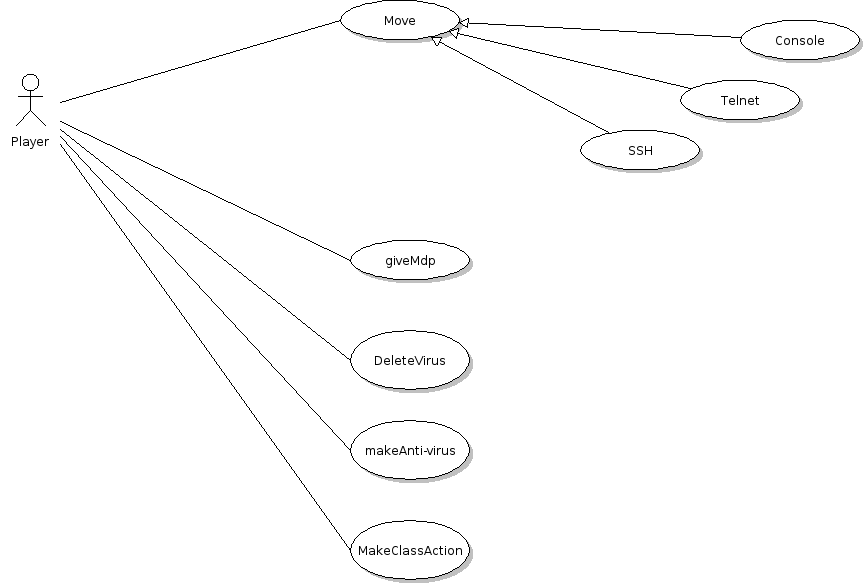
\includegraphics[width=16cm]{report/usecaseEduram.png}
\end{figure}

On peut voir dans ce diagramme que le joueur est le seul acteur dans ce jeu et qu'il à le choix de faire plusieurs actions telle que se déplacer, donner un mot de passe, supprimer des virus, créer un anti-virus ou encore effectuer son action de classe (Rôle).

\subsection{Diagramme de classes}
\begin{figure}[!h]
   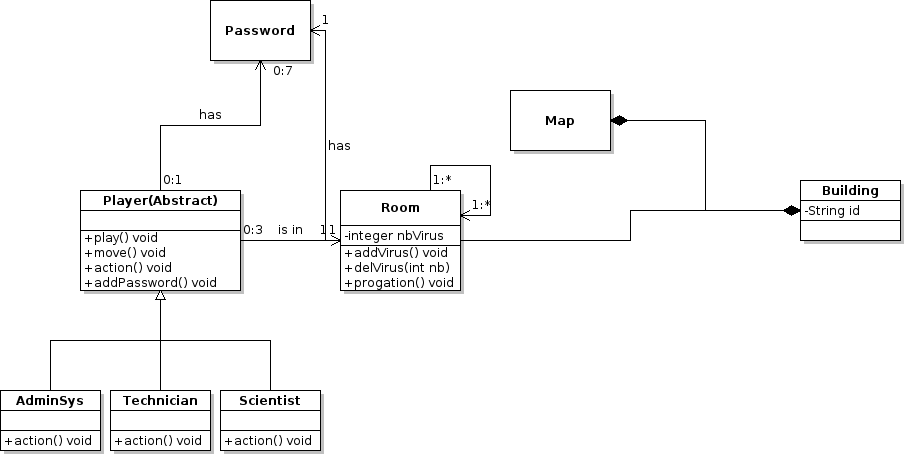
\includegraphics[width=16cm]{report/eduramClasses.png}
\end{figure}
 \pagebreak
Le diagramme de classe précédent représente seulement les classes importantes au niveau algorithmique du jeux. On peut ainsi voir les classes de Joueurs
, la carte ou plateau (map) qui est composée de Bâtiments eux mêmes composés de salles. On peut aussi voir la classe Password qui est une représentation des mot de passe d'accès au salles (la pile de carte joueur dans le jeu original).

\subsection{Diagrammes de séquences}

Nous avons décidé de réaliser plusieurs diagrammes de séquence pour représenter certaines phases importantes du jeu.

\begin{figure}[!h]
   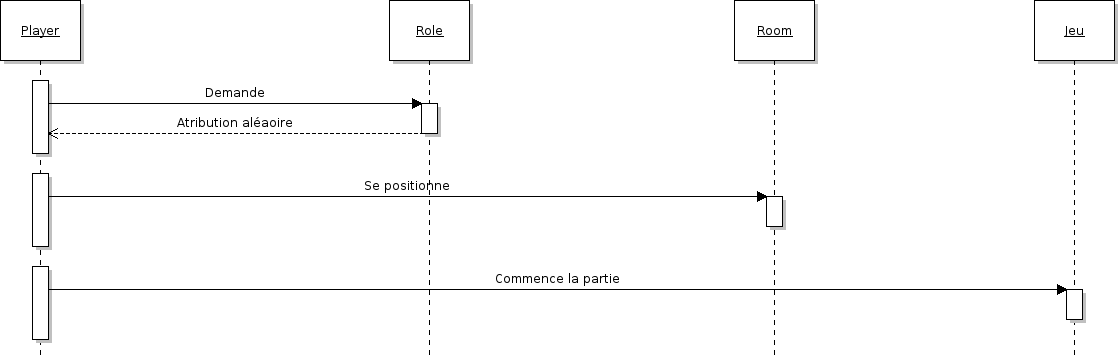
\includegraphics[width=16cm]{report/DiagrameSequenceDebutPartie.png}
   \caption{Ce diagramme représente le début d'une partie, ou le joueur reçoit un rôle, est positionné dans la salle de départ et commence la partie.}
\end{figure}


\pagebreak
\begin{figure}[!h]
   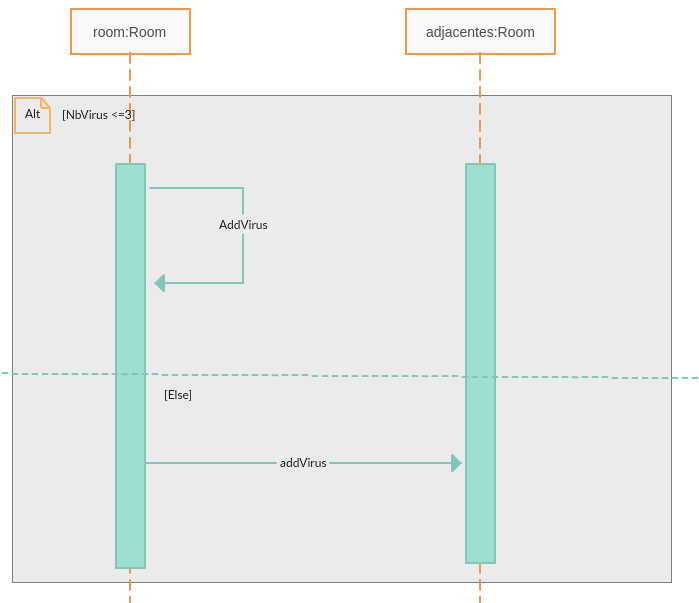
\includegraphics[width=16cm]{report/SequenceEruption.png}
   \caption{Le diagramme ci-dessus représente une éclosion de virus. En effet dans le jeu si il y a déjà 3 virus dans une salle, on ne peut pas rajouter de virus dans cette salle. Par contre un virus est ajouté à toute les salles adjacentes à cette salle. }
\end{figure}

\pagebreak
\begin{figure}[!h]
   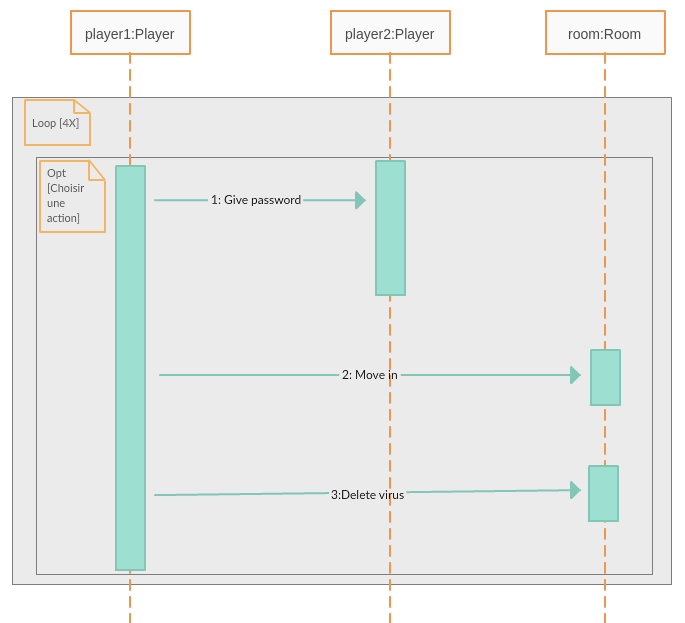
\includegraphics[width=16cm]{report/SequenceTourJoueur.png}
   \caption{Le diagramme ci-dessus représente le tour d'un joueur. Un joueur peut faire 4 actions par tour au choix parmi le déplacement, le don de mot de passe ou encore la suppression d'un virus. }
\end{figure}
\pagebreak
\part{Améliorations possibles}

En développant ce projet nous avons pensé à plusieurs idées d'améliorations. En effet on pensait pouvoir mettre plusieurs types de virus avec des comportements différents, mais ça posait plusieurs problèmes au niveau équilibrage du jeu
Et nous aurions passé plus de temps à réfléchir à la façon d'équilibrer les virus plutôt qu'à les implémenter.

Il peut aussi être possible de rajouter un nouveau rôle de joueur qui serait "Hacker" en effet ce nouveau joueur ne jouerait pas en coopération avec les autres joueurs mais bel et bien contre eux et avec "le jeu"
Cette amélioration aurait été très amusante à mettre en place, mais elle aurait complètement bouleversé le gameplay et nous aurions du revoir une grande partie de l'implémention.

La mise en place du jeu en réseau aurait pu être faisable. En plus grâce à la mise en place du modèle MVC que l'on à fait il n'aurait pas été très compliqué de faire la mise en réseau du jeu. Mais pour faire 
un jeu en ligne cela nécessitait la création d'un serveur et d'un protocole pour les échanges de données. Le client aurait été complètement modifié dans la mesure ou il aurait simplement envoyé des requêtes TCP au serveur et interprété les résultats reçus pour simplement les afficher.
Toutes les vérifications doivent se faire coté serveur et le client n'est en fait qu'un afficheur (Si on commence à contrôler des données sensibles dans le client, les joueurs peuvent trop facilement tricher en modifiant le code du client.).
Cette partie reste, pour nous encore un espoir et sera peut être implémentée car elle nous semble la plus intéressante au niveau programmation. Mais elle nécessite toute fois un gros refactoring de code.

Et enfin nous avions aussi pensé à porter notre jeu pour android. Grâce au modèle MVC, il peut être très simple de créer l'application android. Il nous suffirait seulement de remplacer JavaFX.

\pagebreak
\part{L'implémentation}
Une fois l'étape de conception du projet finalisé, nous avons pu commencer l'implémentation collaborative grâce à Git. Notre objectif de rendre un projet fonctionnel et propre au niveau du code. Dans l'état actuel des choses nous avons une interface graphique affichant un groupe de building contenant des "rooms".

\begin{figure}[!h]
\includegraphics[width=15cm]{report/screenPlateau.png}
\end{figure}

Il nous reste donc à gérer les interactions avec le joueur et rendre l'interface plus jolie.
Au final ce projet nous aura permit de découvrir une nouvelle librairie pour interface graphique et d'améliorer notre connaissance de la programmation orientée objet. Il va de soit que le projet va encore beaucoup évoluer d'ici le rendu et nous tiendrons à jour la documentation pour permettre une meilleur compréhension de notre démarche.

\end{document}
